% ==============================================================================
% LAB 119
% UNDERSÖKNING AV RC-KRETS
% ------------------------
%
% Author:
% Jonas Sjöberg     <tel12jsg@student.hig.se>
% Oscar Wallberg    <tco13owg@student.hig.se>
%
% License:
% Creative Commons Attribution-NonCommercial-ShareAlike 4.0 International
% See LICENSE.md for full licensing information.
% ==============================================================================

\section{Uppmätning av Bode-diagram}\label{bode}

\subsection{Experimentuppställning}\label{}
% ------------------------------------------------------------------------------
En så kallad experimentplatta eller ``breadboard'' används för att konstruera
kretsen som illustreras i Figur~\ref{fig:rc-schema}.  \par För att generera en
sinusformad signal används signalgeneratorn \texttt{HP33120A}, vars utgång
kopplas genom en BNC-förgrening till oscilloskopet \texttt{Agilent 54621A} och
genom en BNC- banankontaktadapter, med ``banankablar'' till breadboardplattans
skruvterminaler.  \par Oscilloskopets första kanal visar signalen från kretsens
ingång, punkten \texttt{Vout} i Figur~\ref{fig:rc-schema}. Samma punkt utgör
signalgeneratorns utgång och vid några mätningar användes en T-koppling av
BNC-kablar för att mata signalgeneratorns utgång till både experimentkopplingen
och oscilloskopet.  En oscilloskopprob är ansluten till oscilloskopets andra
kanal. Proben kopplas till kretsens utgång, punkten \texttt{Vout} i
Figur~\ref{fig:rc-schema} med en oscilloskop-prob. Proben ställs till att dämpa
med en faktor av 10:1 och den vertikala skalan justeras en dekad nedåt, så att
båda kanalerna visas med samma skalfaktor.
\par Impedansskillnaden mellan signalgenerator, kablage och mätutrustning antas
vara hög nog för att inte ha någon avgörande inverkan på mätresultaten. Detta
återkommer i Sektion~\ref{impedans}.


\begin{figure}\label{fig:rc-schema}
  \centering
  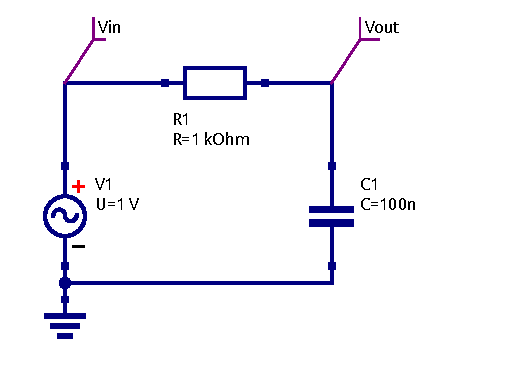
\includegraphics[width=0.8\linewidth]{sim/ee466_lab-4_prj/uppgift-0_schema}
  \caption[Schematisk ritning av labbkoppling, första ordningens RC-filter.]
  {Schematisk ritning av labbkoppling, första ordningens RC-filter.}
\end{figure}

De värden som presenteras i rapporten uppmättes med ett analogt 2-kanals
oscilloskop \texttt{Hitachi V-252} med en bandbredd på \SI{20}{\MHz}.  Signalen
genererades av en hemmabyggd egendesignad signalgenerator.  Kopplingsscheman
till signalgeneratorn återfinns i Figur~\ref{fig:siggen-schem-1} och
Figur~\ref{fig:siggen-schem-2} i Sektion~\ref{appendix}).
Stabiliteten och precisionen hos signalgeneratorn lämnar en del att önska,
kontrollerna är väldigt känsliga och oscilloskopet har ingen frekvensräknare
eller någon direkt visning av amplituden.
likaså är oscilloskopet inte särskilt lättanvänt. Avläsning måste ske
``manuellt'' genom att divisionerna på oscilloskopskärmen räknas och
multipliceras med vald tidbas eller vertikal förstärkning.

För de faktiska mätningarna användes en hemmabyggd signalgenerator (se
Figur~\ref{fig:siggen-schem-1} och Figur~\ref{fig:siggen-schem-2} i
Sektion~\ref{appendix}).
\par Signalgeneratorns amplitud ställs till $1 V_{pp}$. Oscilloskopet som aprecision används en \texttt{Flluke 8600A} Multimeter för att mäta amplituden
som då utrycks i RMS. Sambandet mellan ``topp-till-topp''-värdet och RMS-värdet
utrycks i ekv.~\eqref{eq:amp-rms}:

\begin{equation}\label{eq:amp-rms}
  \begin{split}
    $U_{RMS}      &= \dfrac{\nicefrac{V_{pp}}{2}}{\sqrt{2}}  \\
    $U_{in}_{RMS} &= \dfrac{1}{\sqrt{2}} = \SI{0.354}{\volt} \\
  \end{split}
\end{equation}



\subsection{Beräkning}
% ------------------------------------------------------------------------------
Brytfrekvensen $f_1$ defineras som den frekvens då signalen har dämpats med
\SI{3}{\dB} och beräknas från ekv.~\eqref{eq:transfer2} enligt:

\begin{equation}\label{eq:cutoff}
  f_1 = \dfrac{1}{2 \pi R C} \si{\Hz}
\end{equation}

För kopplingen med komponentvärden enligt Figur~\ref{fig:rc-schema} beräknas
brytfrekvensen $f_1$ enligt ekv.~\eqref{eq:cutoff2}:

\begin{equation}\label{eq:cutoff2}
  \begin{split}
    f_1 &= \dfrac{1}{2 \pi \times \SI{1}{\kohm} \times \SI{100}{\nano\farad}} \si{\Hz} \\
        &= \dfrac{1}{2 \pi \times \num{1e3} \times \num{100e-6}} \si{\Hz}              \\
        &= \dfrac{10^6}{2 \pi \times 10^3 \times \num{100}} \si{\Hz}                   \\
    f_1 &= \SI{1.591549431}{\kHz}
  \end{split}
\end{equation}

Vilket ger svaret i \eqref{eq:cutoff3}; signalen dämpas med \SI{3}{\dB} vid
filtrets brytfrekvens $f_1 \approx \SI{1.592}{\kHz}$, varvid den ``rullas av''
med \SI{20}{\dB} per dekad (frekvenshöjning med en faktor av 10). 

\begin{equation}\label{eq:cutoff3}
  \begin{split}
    f_1 &= \SI{1.591549431}{\kHz} \\
    f_1 &\approx \SI{1.592}{\kHz} \\
  \end{split}
\end{equation}


\subsection{Mätresultat}
% ------------------------------------------------------------------------------

\begin{longtable}[c]{@{}ccccc@{}}
  \toprule\addlinespace
    \begin{tabular}{cc}$\text{Frekvens}        \\ (\si{\hertz})$   \end{tabular}
  & \begin{tabular}{cc}$U_{ut}                 \\ (\si{\volt})$    \end{tabular}
  & \begin{tabular}{cc}$U_{ut}/U_{in}          \\ (\si{\volt})$    \end{tabular}
  & \begin{tabular}{cc}$20 \log{U_{ut}/U_{in}} \\ (\si{\dB})$      \end{tabular}
  & \begin{tabular}{cc}$\phi                   \\ \text{(grader)}$ \end{tabular}
  \\\addlinespace
  \midrule\endhead
   100 & 1.004 & 1.004 & \SI{ 34.67}{\milli} & -3.6 \\\addlinespace 
   200 & 0.998 & 0.998 & \SI{-17.38}{\milli} & -7.2 \\\addlinespace 
   300 & 0.997 & 0.997 & \SI{-26.09}{\milli} & -10  \\\addlinespace % 1mS
   500 & 0.990 & 0.990 & \SI{-87.29}{\milli} & -17  \\\addlinespace % 0.1mS   ???
   700 & 0.984 & 0.984 & \SI{-140.1}{\milli} & -23  \\\addlinespace % 0.15mS  ???
  1000 & 0.958 & 0.958 & \SI{-372.7}{\milli} & -32  \\\addlinespace % 0.1mS   ???
  1200 & 0.952 & 0.952 & \SI{-427.3}{\milli} & -37  \\\addlinespace % 60uS
  1300 & 0.949 & 0.949 & \SI{-454.7}{\milli} & -39  \\\addlinespace % ????
  1500 & 0.943 & 0.943 & \SI{-509.8}{\milli} & -43  \\\addlinespace % 40uS
  1600 & 0.940 & 0.940 & \SI{-537.4}{\milli} & -45  \\\addlinespace % 35uS
  1700 & 0.938 & 0.938 & \SI{-555.9}{\milli} & -47  \\\addlinespace % ?????
  1800 & 0.936 & 0.936 & \SI{-574.5}{\milli} & -48  \\\addlinespace % 35uS
  1900 & 0.934 & 0.934 & \SI{-593.1}{\milli} & -50  \\\addlinespace % 35uS
  2000 & 0.932 & 0.932 & \SI{-611.7}{\milli} & -51  \\\addlinespace % ????
  \bottomrule
  \addlinespace
  \caption[]{Mätresultat för kretsen i Figur~\ref{fig:rc-schema}.}
  \label{bode-table}
\end{longtable}


% TODO: Bode-diagram för frekvensgång.

% TODO: Bode-diagram för Fasförskjutning.


\subsection{Simulering}
% ------------------------------------------------------------------------------
För verifiering och visualisering av den teoretiska beräkningen körs en
\texttt{SPICE}-simulering av kretsen i det GPL-licensierade open source
programmet \texttt{Qucs}\footnote{\url{http://qucs.sourceforge.net/}}.
Simuleringsuppställningen och resultatet återfinns i
Figurer~\ref{fig:bode-sim-ac}, Figur~\ref{fig:bode-sim-tran} och
Figur~\ref{fig:bode-sim-param}.

\begin{figure}\label{fig:bode-sim-ac}
  \centering
  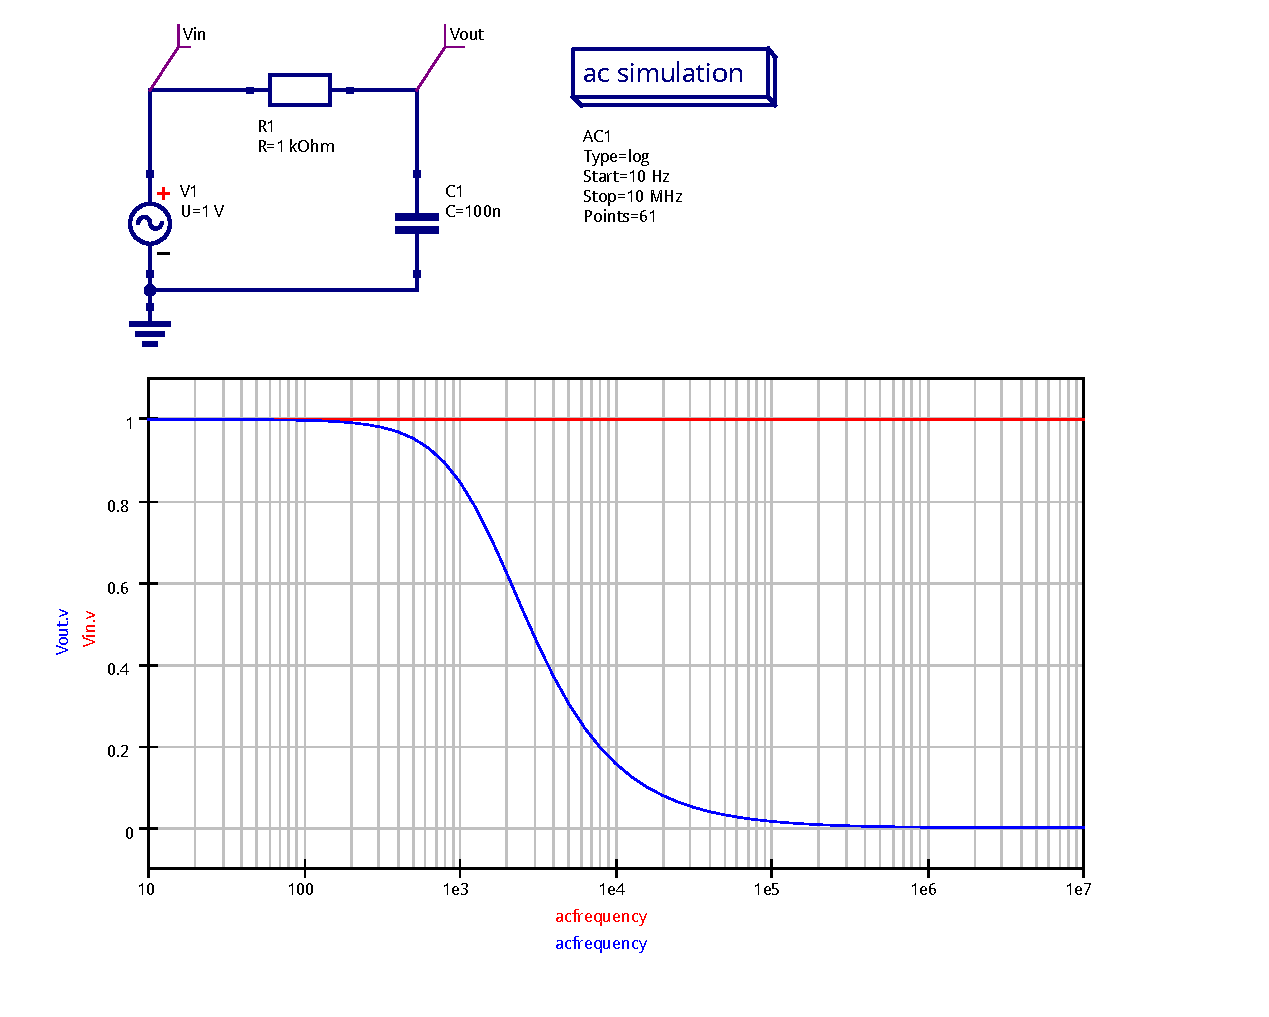
\includegraphics[width=\linewidth]{sim/ee466_lab-4_prj/uppgift-1_ac}
  \caption[] {Simulering av kretsens frekvensåtergivning.}
\end{figure}

\begin{figure}[ht]\label{fig:bode-sim-tran}
  \centering
  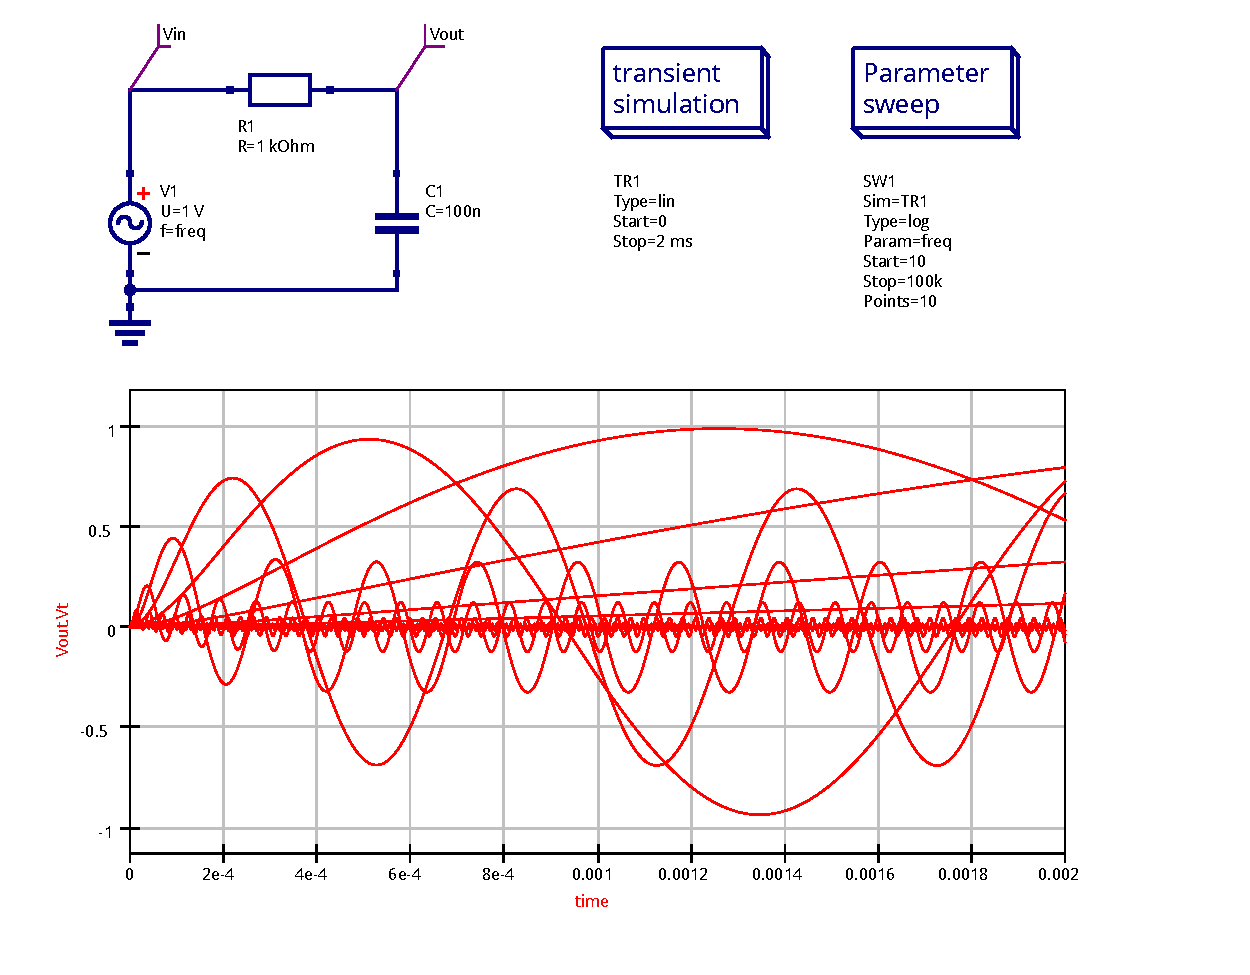
\includegraphics[width=\linewidth]{sim/ee466_lab-4_prj/uppgift-1_tran}
  \caption[] {Simulering av kretsen i tidsdomänen för olika frekvenser av $V_1$.}
\end{figure}

\begin{figure}[ht]\label{fig:bode-sim-param}
  \centering
  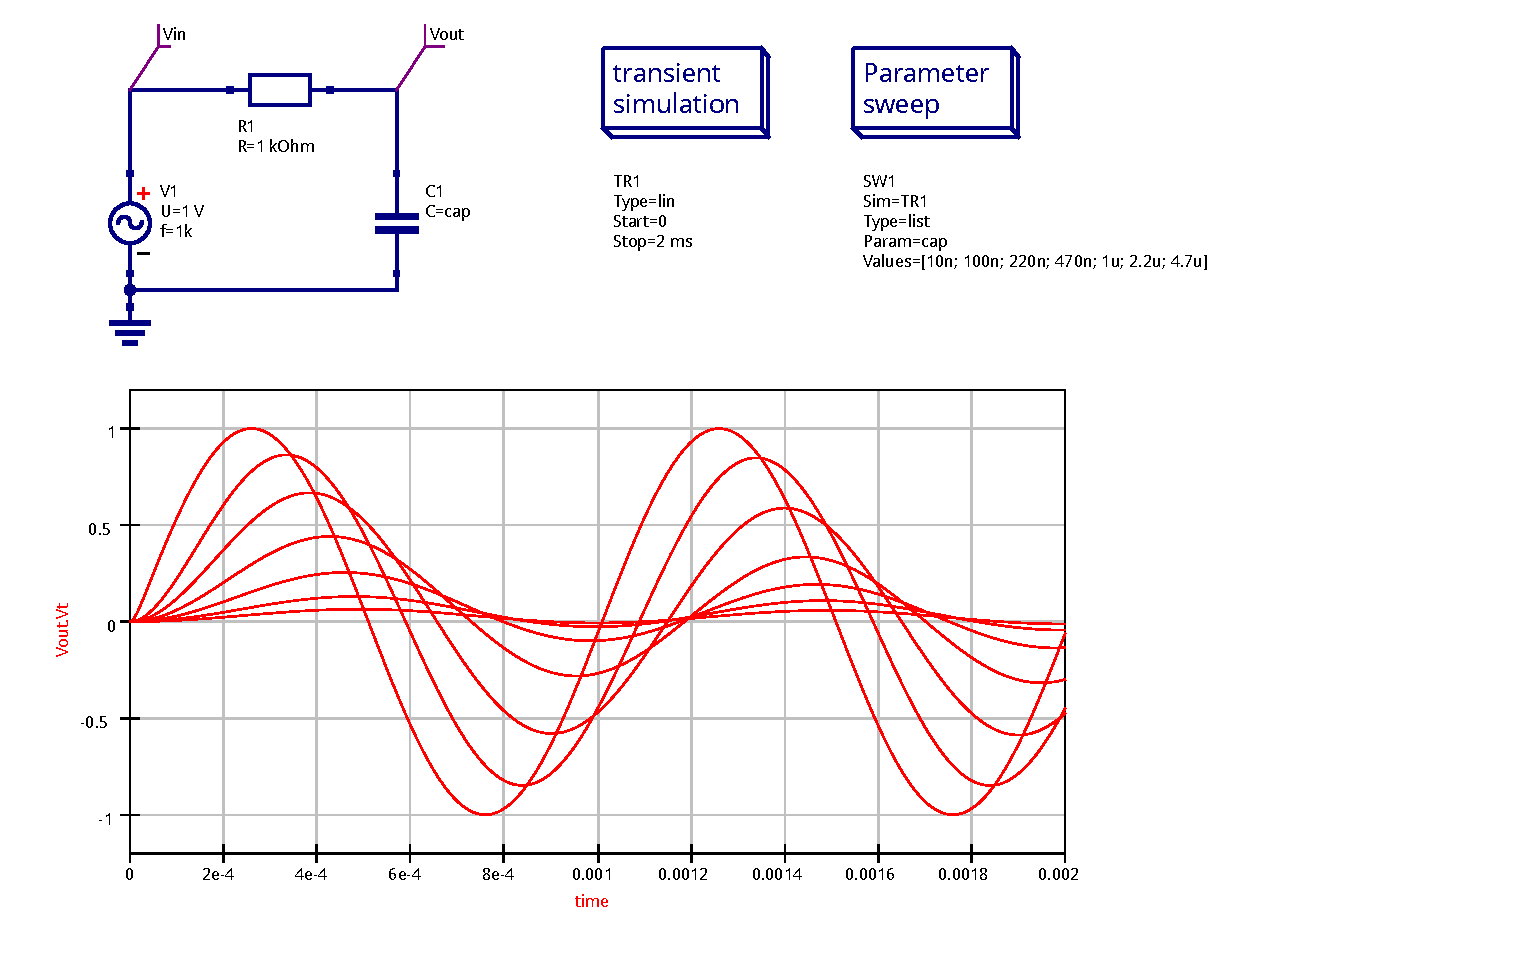
\includegraphics[width=\linewidth]{sim/ee466_lab-4_prj/uppgift-1_param}
  \caption[] {Simulering av kretsen i tidsdomänen för olika värden av $C_1$.}
\end{figure}


\subsection{Kommentar}\label{}
% ------------------------------------------------------------------------------
% TODO:


